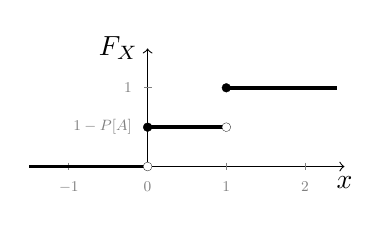
\begin{tikzpicture}
    \draw[->] (-1.5, 0) -- (2.5, 0) node[below] {$x$};
    \draw[->] (0, 0) -- (0, 1.5) node[left]{$F_X$};
    \foreach \x in {-1, ..., 2} {
        \draw [gray] (\x, 0.05) -- ++(0, -.1) ++(0, -.15) node [below, outer sep=0pt, inner sep=0pt, scale=0.6] {\small\(\x\)};}
    \foreach \y in {1} {
        \draw [gray] (0.05, \y) -- ++(-.1, 0) ++(-.15, 0) node [left, outer sep=0pt, inner sep=0pt, scale=0.6] {\small\(\y\)};}
    \draw [gray] (0.05, 0.5) -- ++(-.1, 0) ++(-.15, 0) node [left, outer sep=0pt, inner sep=0pt, scale=0.6] {\small\(1-\mathbb{P}[A]\)};
    \draw[draw=black,line width=1.3pt] (-1.5,0) -- (0,0);
    \draw[draw=black,line width=1.3pt] (0,0.5) -- (1,0.5);
    \draw[draw=black,line width=1.3pt] (1,1) -- (2.4,1);
    \filldraw[draw=black,line width=0.1pt,fill=white] (0,0) circle[radius=1.6pt];
    \filldraw[draw=black,line width=0.1pt,fill=black] (0,0.5) circle[radius=1.6pt];
    \filldraw[draw=black,line width=0.1pt,fill=white] (1,0.5) circle[radius=1.6pt];
    \filldraw[draw=black,line width=0.1pt,fill=black] (1,1) circle[radius=1.6pt];
\end{tikzpicture}